Abbiamo scelto di semplificare la superchiave dell'entità "Costo di spedizione", composta da 4 attributi, aggiungendo l'attributo "Codice".


\noindent\makebox[\textwidth]{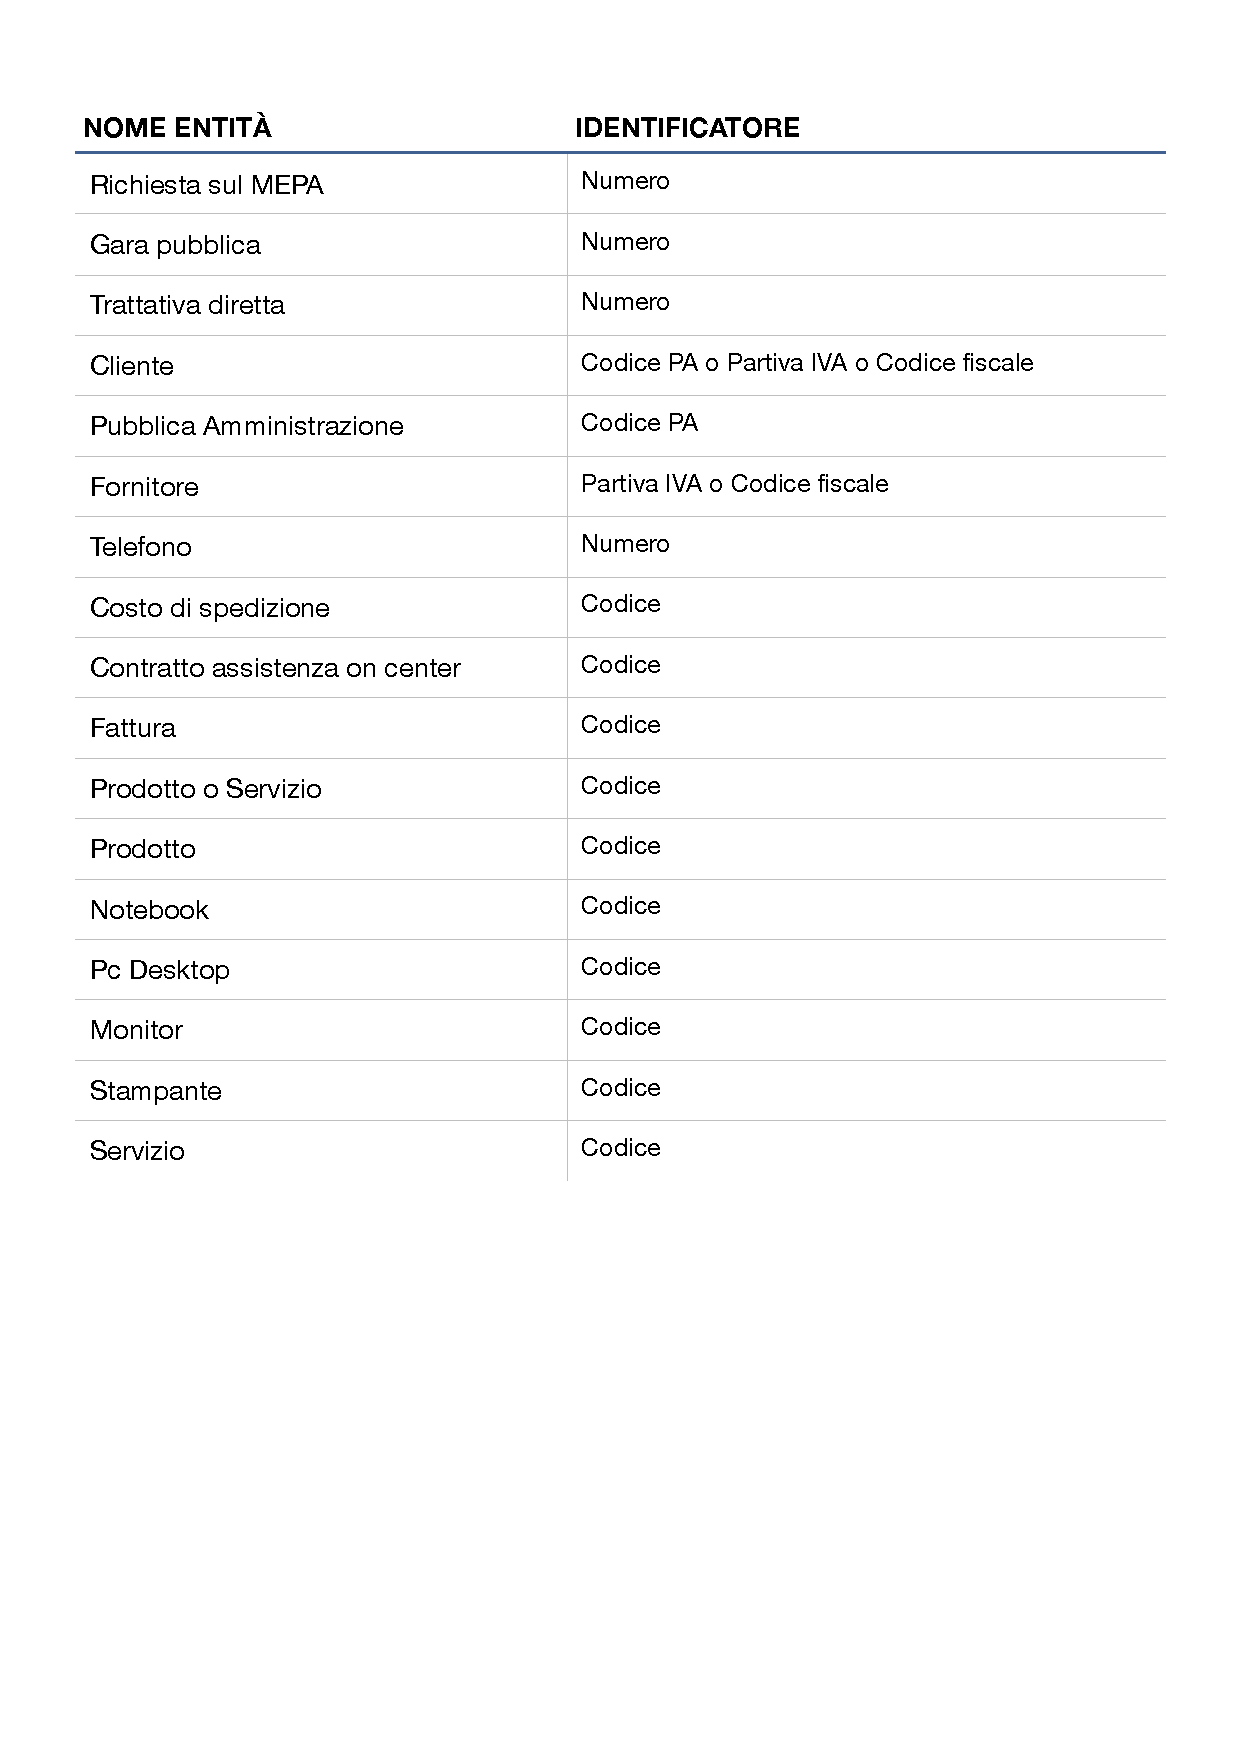
\includegraphics[width=1.1\linewidth, trim=0 8cm 0 0]{./pdf/identificatori_principali.pdf}}



% \begin{table}[H]
% \centering
% \resizebox{.65\textwidth}{!}{%
% \begin{tabular}{|l|l|}
% \hline
% \multicolumn{1}{|c|}{\textbf{NOME ENTIT\'{A}}} & \multicolumn{1}{c|}{\textbf{IDENTIFICATORE}} \\ \hline
% Personaggio        & Nome         \\ \hline
% Missione           & CodiceMiss   \\ \hline
% Abilità            & Nome         \\ \hline
% Oggetto            & Nome         \\ \hline
% Consumo            & CodConsumo   \\ \hline
% Equipaggiamento    & Nome         \\ \hline
% Consumabili        & Nome         \\ \hline
% Oggetti Missione   & Nome         \\ \hline
% Npc Amichevole     & Nome         \\ \hline
% Npc Ostile         & CodNPCOST    \\ \hline
% Transazione        & CodTrans     \\ \hline
% Utente             & Username     \\ \hline
% Prodotto           & Codprodotto  \\ \hline
% Sottoscrizione     & CodSottoscr  \\ \hline
% Pacchetto Oggetti  & CodPacchOgg  \\ \hline
% Espansione         & CodEsp       \\ \hline
% Carta Credito      & numero       \\ \hline
% \end{tabular}
% }
% \end{table}



% \newpage
% \begin{landscape} %inizia un foglio landscape
%
% %include un file pdf che contiene lo schema
% 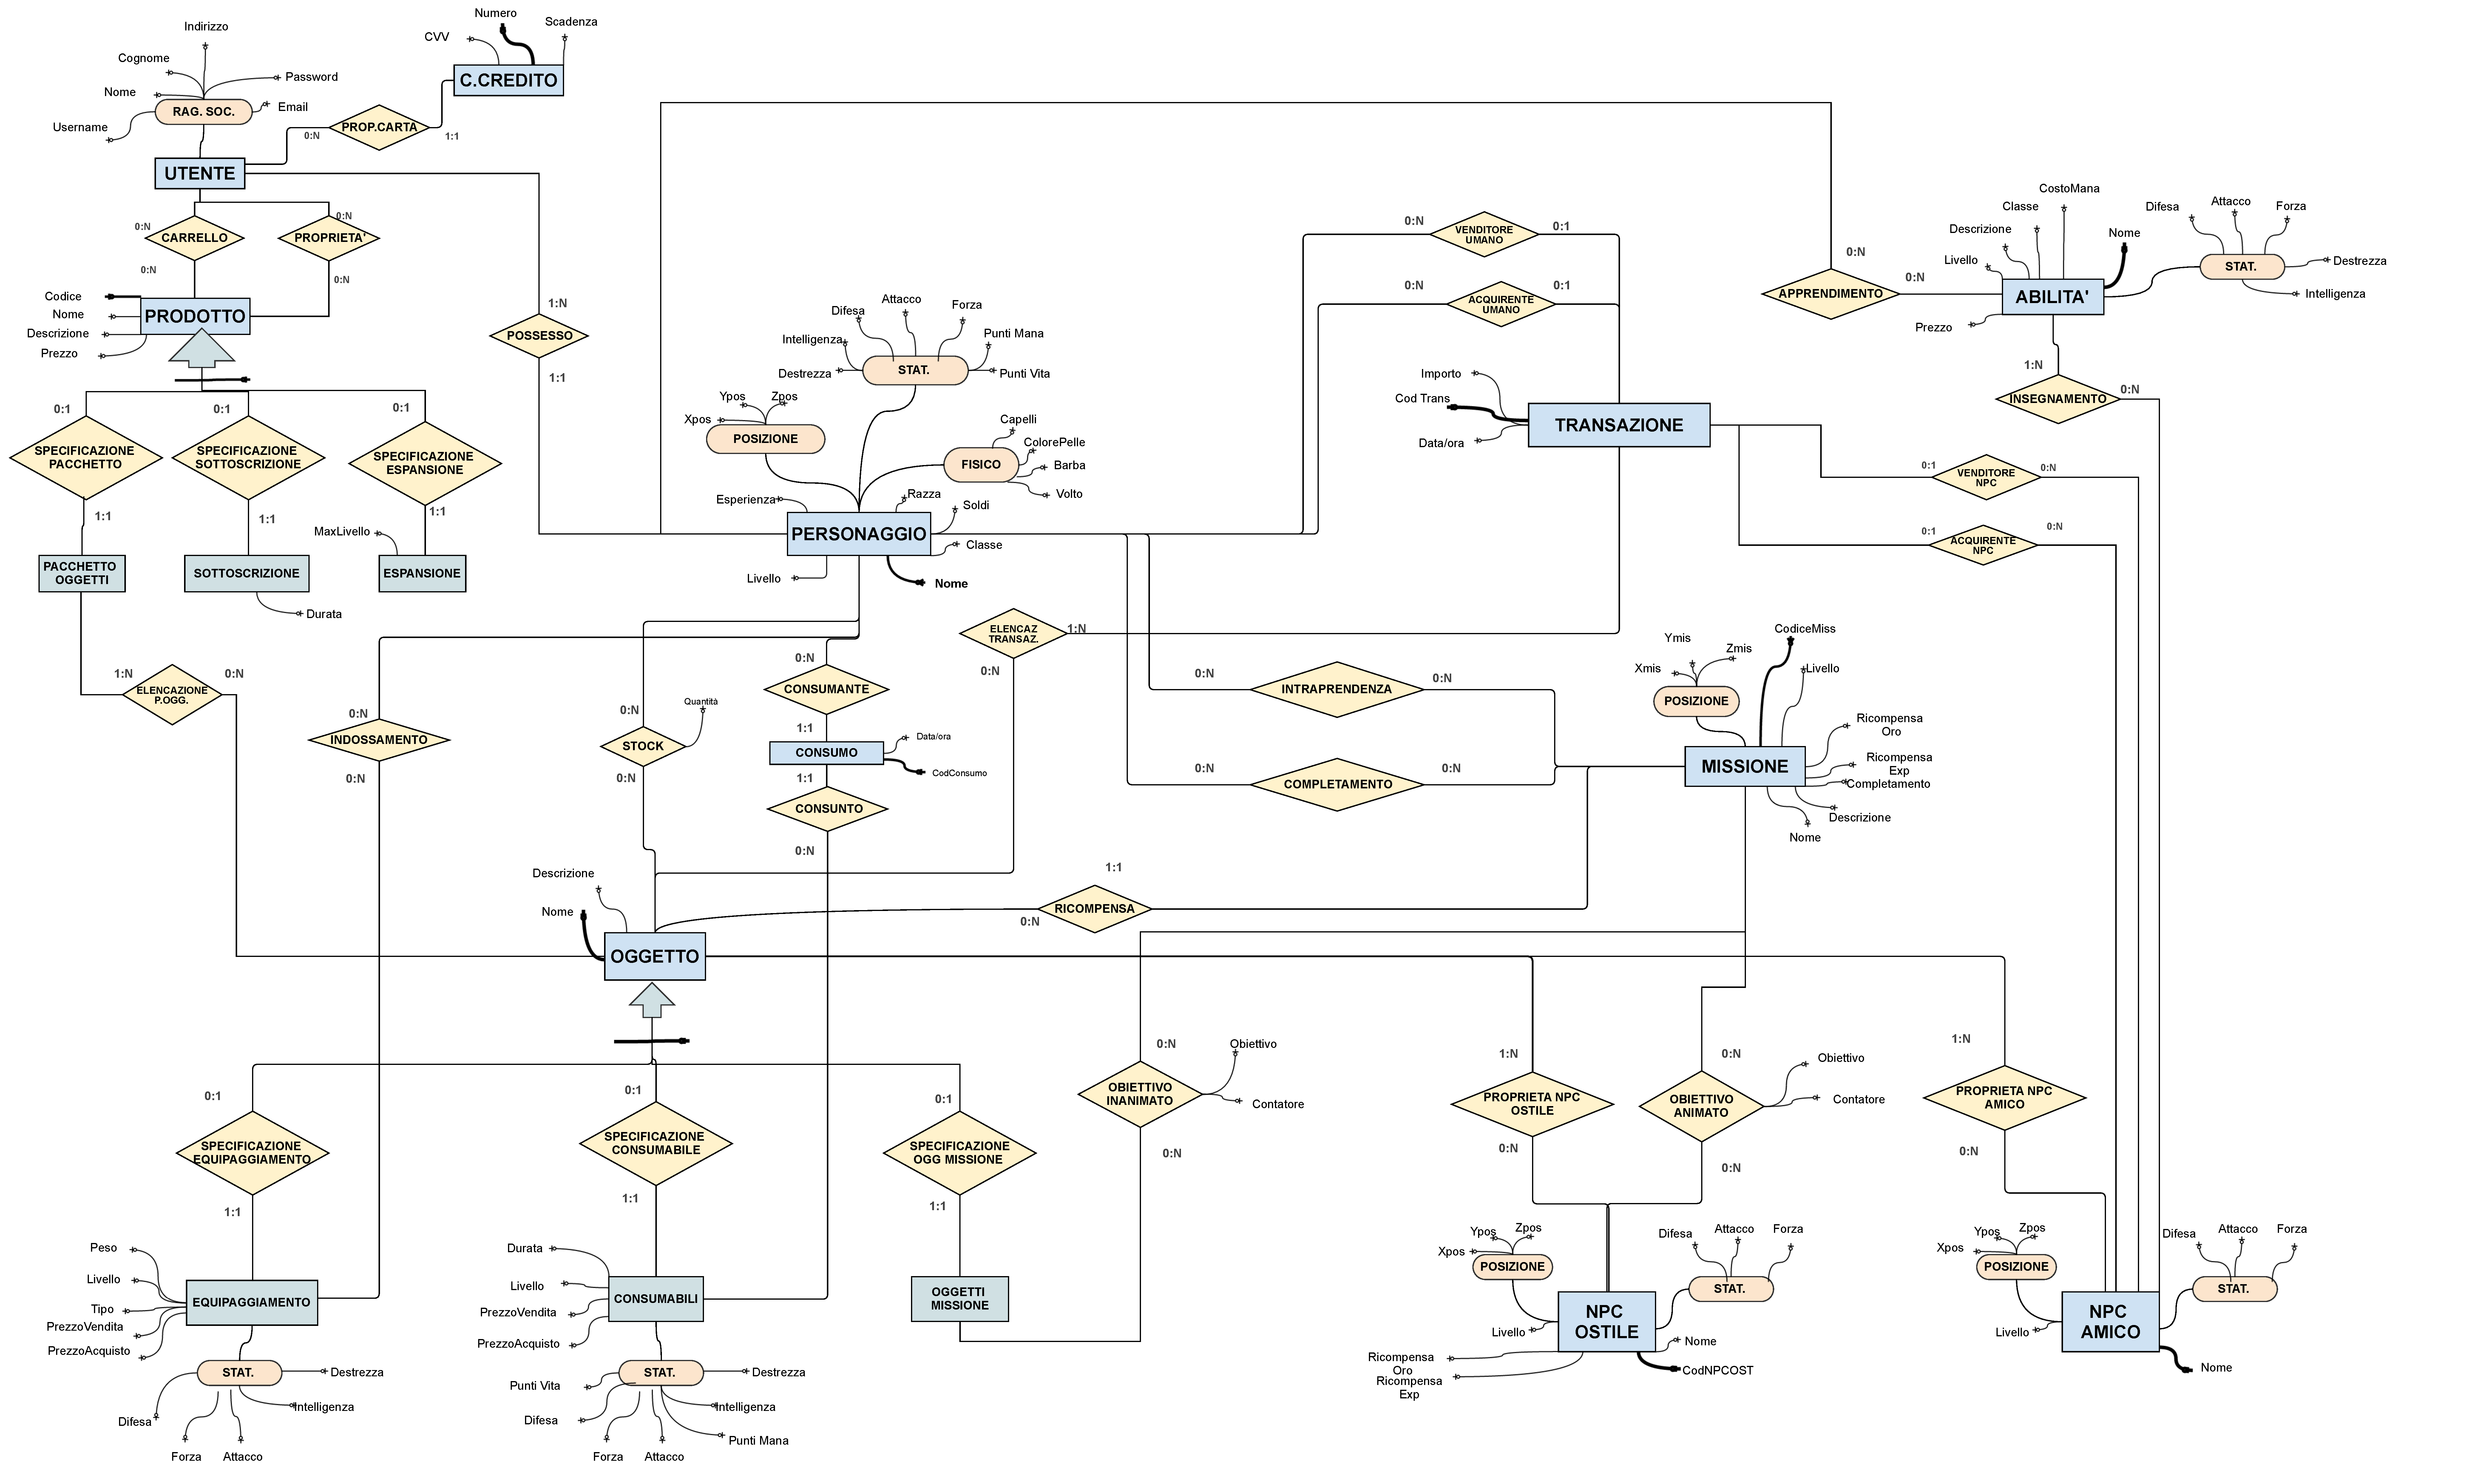
\includepdf[width=270mm, height=210mm, angle=90, keepaspectratio]{./pdf/ristrutturatocarta.pdf}
%
% \end{landscape}
